\documentclass[12pt]{article}

\usepackage[a4paper, total={7in, 10in}]{geometry}
\usepackage[utf8]{inputenc}
\usepackage{amsmath}
\usepackage{enumitem}
\usepackage{siunitx}
\usepackage{graphicx}
\usepackage{hyperref}

\linespread{1.15}

\title{IDATT2104 - Arbeidskrav 1}
\author{Gruppe 18}
\date{\today}

\begin{document}
    \maketitle
    \newpage

    \tableofcontents

    \newpage

    \section{P3 - Sockets, TCP, HTTP og tråder}
    \subsection{Enkel klient/tjener}
    Vi har to programmer. Tjener og klient. De bruker TCP på transportlaget og 
    IPv4 på nettverkslaget for å kommunisere. Programmene fungerer som følger.
    Tjeneren kjører først, og vil så begynne å lytte på en port.
    Vi velger helst en port mellom 49152-65535, som er intervallet for porter som er 
    dynamiske/midlertidig brukt. I vårt tilfelle har vi valgt 54321. Tjeneren venter 
    på en klient som vil koble seg opp.
    
    For denne oppkoblingen vil klienten og tjeneren ha følgende info

    \begin{center}
        \begin{tabular}{|l|l|l|}
            \hline
                 & Klient            & Tjener            \\ \hline
            MAC  & b4:2e:99:34:ef:5f & 08:26:97:e6:7e:50 \\ \hline
            IP   & 94.245.94.80      & 192.168.0.187     \\ \hline
            Port & 41982             & 54321             \\ \hline
        \end{tabular}
    \end{center}
    
    Tjeneren vil så akseptere tilkoblingen med et 
    TCP 3-way handshake. Handshaket går ut på (SYN, SYNACK, ACK), og vises i bildet under.

    \begin{center}
        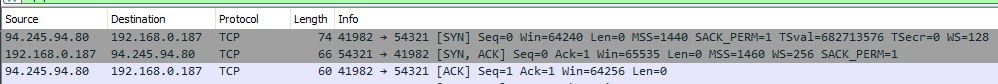
\includegraphics[width=\linewidth]{assets/9GhtNDG.png}
    \end{center}
    
    Her ser vi et TCP 3-way handshake, (SYN, SYNACK, ACK). Tjeneren lytter på
    port 54321, så vi ser at klienten sender en SYN til tjeneren og har sekvensnummer 0.
    Tjeneren svarer med med en SYNACK-pakke som har kvitteringsnummer 1 og sekvensnummer 0.
    Klienten får dette, og svarer tjeneren igjen med en ACK-pakke
    som har sekvensnummer 1 og kvitteringsnummer 1. Dette stemmer overens med et 3-way handshake.

    Tjeneren venter så på at klienten skal sende over data, og når dette skjer vil dataen
    ankomme tjeneren, som så vil sende en ACK-pakke tilbake til klienten. Dataen vil så 
    bli lest av tjeneren, bli behandlet, og tjeneren vil så sende tilbake et svar. I dette 
    tilfellet får tjeneren tilsendt et enkelt regnestykke, og sender tilbake et svar.

    Bildet under vil vise en pakke som går fra klient til tjener, og inneholder et regnestykke.

    \begin{center}
        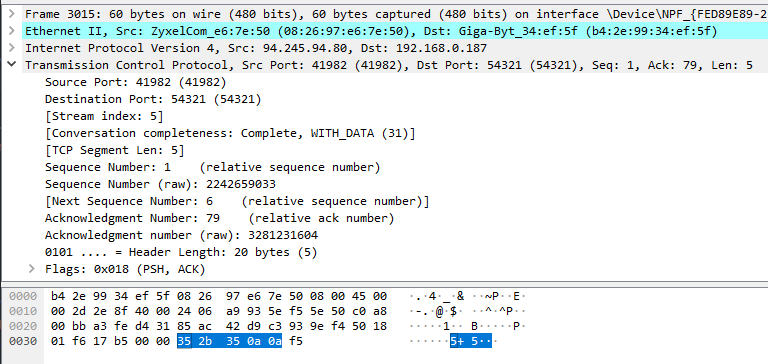
\includegraphics[width=\linewidth]{assets/5K1kvx9.png}
    \end{center}
    
    Her ser vi TCP-flagg som PSH og ACK, i tillegg til sekvensnummer og kvitteringsnummer. 
    Tjeneren behandler så regnestykket og sender tilbake et svar. I programmet ser det slik ut

    \begin{center}
        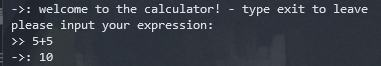
\includegraphics{assets/7j3MtCt.png}
    \end{center}

    Klienten kan så koble seg fra tjeneren ved å skrive inn "exit", som vil begynne 
    nedkoblingen av TCP-tilkoblingen. Dette skjer ved et nytt handshake. Når nedkoblingen 
    begynner, sender klienten en pakke med FIN-flagget satt, til tjeneren. Tjeneren vil sende en 
    pakke med ACK-flagget satt tilbake til klienten for å fortelle at tjeneren vet at klienten vil 
    at tilkoblingen skal avsluttes. Tjeneren sier så også at den ikke lenger vil ha tilkoblingen 
    oppe ved å sende en FIN-pakke til klienten, og klienten vil sende tilbake en ACK-pakke.
    Etter dette er tilkoblingen avsluttet og data vil ikke lenger bli overført.

    Bildet under viser nedkoblingen, etter at klienten har sendt "exit" til tjeneren.

    \begin{center}
        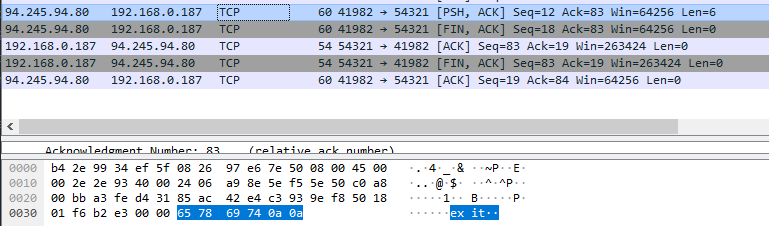
\includegraphics[width=\linewidth]{assets/pYiH4NJ.png}
    \end{center}

    Tabellen under viser sekvens- og kvitteringsnummere for "exit"-meldingen og selve nedkoblingen.

    \begin{center}
        \begin{tabular}{|l|l|l|l|}
            \hline
              & Seq & Ack & Length \\ \hline
            1 & 12  & 83  & 6      \\ \hline
            2 & 18  & 83  & 0      \\ \hline
            3 & 83  & 19  & 0      \\ \hline
            4 & 83  & 19  & 0      \\ \hline
            5 & 19  & 84  & 0      \\ \hline
        \end{tabular}
    \end{center}

    \subsection{Flere klienter samtidig}
    Denne oppgaven bygger bare på den forrige. Individuelle klienter vil ikke merke noe forskjell.
    Tjeneren lager bare en tråd for hver tilkobling, og behandler dem helt individuelt. Det eneste 
    som egentlig blir forskjellig i Wireshark, er at vi kan se flere tilkoblinger til samme port 
    hos tjeneren istedenfor bare én.
    
    \subsection{Enkel webtjener med nettleser som klient}

    I denne oppgaven bruker vi TCP på transportlaget over IPv4 på nettverkslaget. Klienten kobler opp 
    til serveren med et 3-way TCP handshake til serveren, deretter sender en HTTP GET 
    request til serveren. Serveren vil så lese headerne fra GET-requesten, 
    og så sende tilbake en HTTP-respons med HTML-filen som inneholder listen med headere. Så vil 
    TCP-koblingen avsluttes i nok et handshake som består av FIN og ACK-pakker. 

    Tabellen under viser IP, MAC og porter for klient og tjener.
    
    \begin{center}
        \begin{tabular}{|l|l|l|}
            \hline
                 & Klient            & Tjener            \\ \hline
            MAC  & b4:2e:99:34:ef:5f & 08:26:97:e6:7e:50 \\ \hline
            IP   & 94.245.94.80      & 192.168.0.187     \\ \hline
            Port & 57186             & 80                \\ \hline
        \end{tabular}
    \end{center}

    Bildet under viser et skjermklipp fra Wireshark. Bildet viser oppkobling og nedkobling av TCP, og 
    overføring av data, og mye av informasjonen for tilkoblingen. 
    Nederst på bildet viser vi den første pakken, altså SYN pakken øverst på lista. Her ser vi
    sekvensnummer som er 0, kvitteringsnummer som er 0. TCP-flaggene viser at SYN flagget er satt, 
    men ingen andre. Vi kan se på lista hvordan sekvensnummerne og kvitteringsnummerne øker etter hvert
    som flere pakker blir sendt, som er forventet. For den valgte pakken kan vi se IP, porter og 
    MAC-addresser, som tilsvarer det som står på tabellen over. 
    
    \begin{center}
        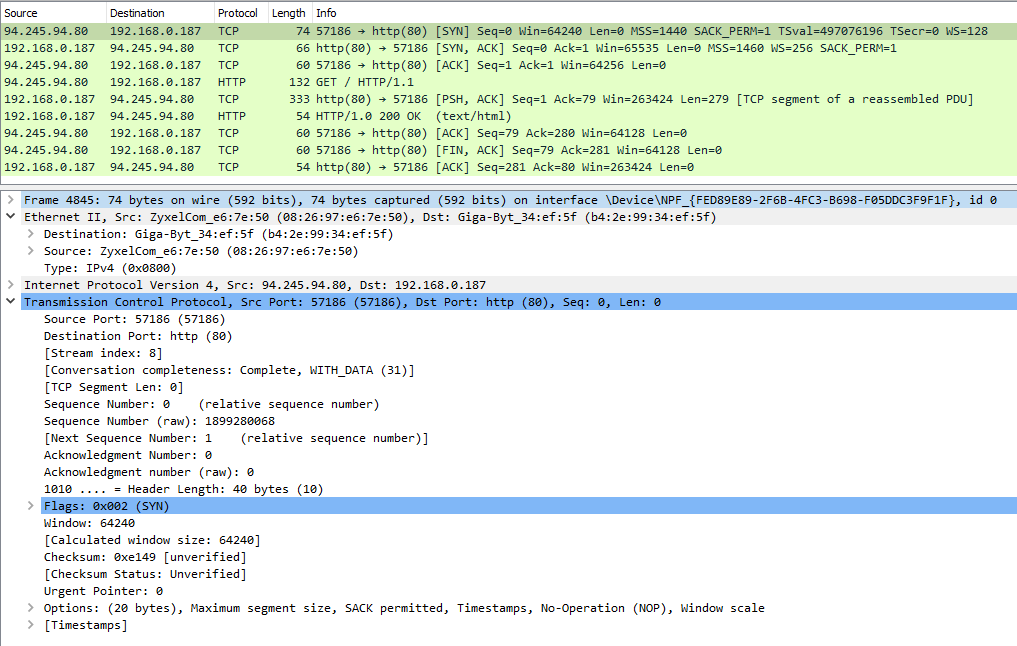
\includegraphics[width=7in]{assets/z4qWyHn.png}
    \end{center}
    
    \section{P4 - UDP, TLS, ASIO}
    \subsection{UDP kalkulator}
    Denne oppgaven har to programmer, begge bruker UDP på transportlaget, og IPv4 på nettverkslaget.
    For klienten så er virkemåten for programmet ganske likt som TCP-kalkulatoren. Forskjellen er at 
    bruken av UDP kan gjøre at pakker ikke når fram. Dette er fordi UDP ikke har en oppkobling som 
    TCP. Det er ikke noe 3-way handshake. Heller ingen ACK-pakker for å finne ut om pakker nådde frem.
    Klienten vil prøve å sende en melding til tjeneren. Dersom 
    meldingen ikke når frem til tjeneren, får vi ikke noe svar tilbake. Dermed er det viktig å passe på 
    at vi bare venter på svar fra tjeneren i en viss tid. Dersom vi går over den tiden, kan 
    vi anta at pakken ikke nådde frem, eller at pakken fra tjeneren til klienten ikke nådde frem. 
    UDP-pakker er mindre enn TCP-pakker, noe som gjør dem raskere. De har ingen sjekker for å finne 
    ut om pakkene nådde fram eller ikke, noe som gjør dem litt mindre pålitelige som TCP.

    Vi kan se på hva slags data som blir sendt mellom programmene via Wireshark.
    For UDP-kalkulatoren i dette tilfellet, vil tjeneren og klienten ha følgende info

    \begin{center}
        \begin{tabular}{|l|l|l|}
            \hline
                 & Klient            & Tjener            \\ \hline
            MAC  & b4:2e:99:34:ef:5f & 08:26:97:e6:7e:50 \\ \hline
            IP   & 94.245.94.80      & 192.168.0.187     \\ \hline
            Port & 53968             & 54321             \\ \hline
        \end{tabular}
    \end{center}
    
    Under ser vi et skjermklipp fra Wireshark. Der ser vi først og fremst at det er mye mindre 
    som skjer i forhold til TCP. Det er ingen 3-way handshake. Det er bare enkle og små pakker
    som klienten først prøver å sende til tjeneren. Deretter behandler tjeneren meldingen som
    den mottar, og prøver å sende en melding tilbake til klienten. 

    \begin{center}
        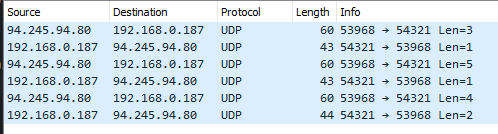
\includegraphics{assets/Yz1XfZv.png}
    \end{center}

    Det neste bildet viser et skjermklipp fra selve klientprogrammet.
    
    \begin{center}
        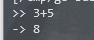
\includegraphics{assets/8kkg5An.png}
    \end{center}

    Bildet viser at vi sender et regnestykke, og får et svar. De neste to bildene viser hvordan 
    pakkene for dette faktisk ser ut. Dersom vi ser på bildet med listen av pakker, vil dette 
    være de to første pakkene.

    \begin{center}
        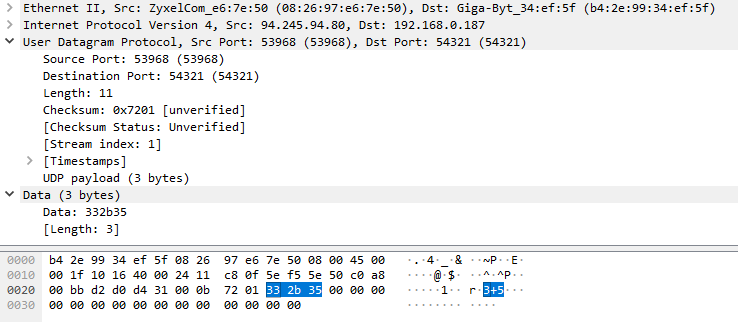
\includegraphics[width=\linewidth]{assets/46A9fBV.png}
    \end{center}
    
    Dette er pakken fra klienten til tjeneren. Vi kan se at porter, IP og MAC-addresse stemmer 
    overens med tabellen over. Vi ser at pakkene er mye mindre enn en TCP-pakke. Det som er 
    markert i blått er den dataen vi sender over. I dette tilfellet er det $3+5$, noe som vi 
    også ser fra skjermklippet fra klientprogrammet. Så kan vi se på hvordan det ser ut når 
    vi får et svar fra tjeneren på bildet under.

    \begin{center}
        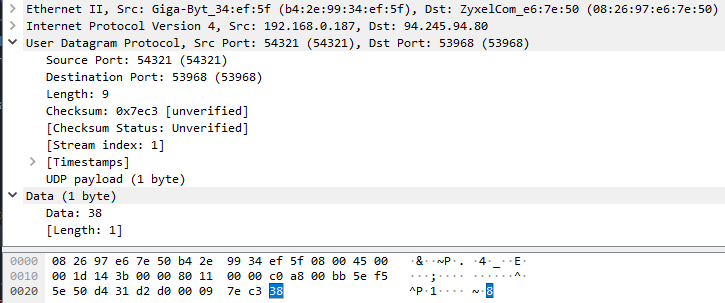
\includegraphics[width=\linewidth]{assets/3oYp41n.png}
    \end{center}

    På dette bildet ser vi mye av det samme som det forrige. Hovedforskjellen er at dette er 
    pakken fra tjeneren tilbake til klienten. Dataen som blir sendt er igjen markert i blått, og 
    viser at dataen er tallet 8. Dette stemmer igjen overens med skjermklippet fra klientprogrammet,
    i tillegg til den forrige pakken, som sendte over regnestykket $3+5$. 

    Når klienten ønsker, kan en avslutte klientprogrammet ved å skrive "exit", som vil avslutte 
    programmet. I motsetning til TCP-kalkulatoren, er det ingen nedkobling i dette tilfellet, fordi 
    det aldri var noen oppkobling heller. 

    
    \subsection{TLS}
    For denne oppgaven hadde vi noe problemer med å gjøre eksemplet som øvingen ba oss om å gjøre. 
    Dermed bestemte vi oss for å bare skrive om klient/tjener programmet fra P3, men slik at det 
    bruker TLS isteden. Kildekoden for dette kan finnes på \href{https://gist.github.com/IntrntSrfr/f5b8456fbae987d2870b99010cf0865b}{GitHub}

    \url{https://gist.github.com/IntrntSrfr/f5b8456fbae987d2870b99010cf0865b}

    For dette programmet er virkemåten lik som i P3, men vi bruker TLS. For å gjøre dette, er vi 
    først nødt til å generere et sertifikat, og en nøkkel. Dette kan vi gjøre ved å bruke OpenSSL,
    og gir oss en \verb|server.crt| fil og en \verb|server.key| fil som vi kan bruke. Det er enkelt 
    å legge til et selv-signert sertifikat på en server, men ettersom dette ikke er et sertifikat fra
    en Certificate Authority, vil det si at klienter ikke vil stole på sertifikatet. Dette 
    er ikke overraskende, fordi å lage et selv-signert sertifikat kan sammenliknes med å kjøpe en 
    falsk politiuniform fra AliExpress, og så si at man er politi. Altså, det er ikke 
    mye som vil stole på det, fordi det ikke kommer fra en sentral autoritet. Bortsett fra i 
    visse tilfeller, som vi nå skal gå inn på. 

    Selv om det vanligvis er tilfellet at et selv-signert sertifikat ikke kan stoles på, er
    dette bare et lite program for å kun lære om TLS.
    Dermed kan vi få klienten til å stole på sertifikatet, ved å bare legge det til i programmet
    og si at det kan stoles på. Vi kan stole på oss selv, så dette går fint. Programmet vil 
    dermed legge til sertifikatet i sin egen lokale bank med sertifikater som det kan stole på, 
    og dermed vil vi kunne bruke det for å koble opp til tjeneren med TLS.

    Hele poenget med TLS er at data skal være kryptert under overføringen. Det vil si at vi 
    ikke skal kunne åpne Wireshark, klikke på en pakke og se i klartekst hvilke data som er 
    overført. Dette gjøres ved å bruke sesjonsnøkler, private og offentlige nøkler og 
    kryptografisuiter. Sesjonsnøkler blir satt sammen av både klienten og tjeneren ved bruk av 
    to tilfeldige genererte bytestrings som både klienten og tjeneren genererer
    Private og offentlige nøkler får vi via \verb|server.crt| og \verb|server.key| som vi 
    genererer selv. Kryptografisuitene som tilkoblingen bruker blir bestemt under oppkoblingen 
    via TLS-handshake.

    Når vi har gjort dette, er virkemåten lik som i P3, hvor det er en tjener som tar imot regnestykker
    og sender tilbake et svar, og en klient som sender regnestykkene.

    Programmene bruker TCP på transportlaget og IPv4 på nettverkslaget for å 
    kommunisere.

    For denne oppkoblingen vil klienten og tjeneren ha følgende info

    \begin{center}
        \begin{tabular}{|l|l|l|}
            \hline
                 & Klient            & Tjener            \\ \hline
            MAC  & b4:2e:99:34:ef:5f & 08:26:97:e6:7e:50 \\ \hline
            IP   & 94.245.94.80      & 192.168.0.187     \\ \hline
            Port & 52632             & 54321             \\ \hline
        \end{tabular}
    \end{center}
    
    Oppkoblingen vil ha samme (SYN, SYNACK, ACK) 3-way handshake som i P3. 

    \begin{center}
        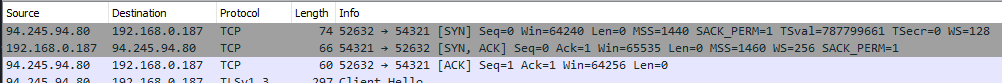
\includegraphics[width=\linewidth]{assets/ce56Xhh.png}
    \end{center}

    Bildet viser for det meste akkurat det samme som for P3, men portene er forskjellige i dette
    tilfellet. Vi ser samme sekvensnummer og kvitteringsnummer for oppkoblingen som i P3. Det 
    som er forskjellen når det kommer til TLS, er at før data vil bli overført, 
    så vil tilkoblingen gjøre et TLS handshake som vist på bildet under. 
    
    \begin{center}
        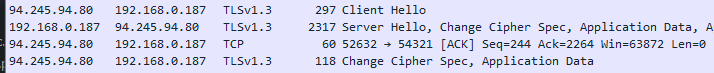
\includegraphics[width=\linewidth]{assets/8kKfzaM.png}
    \end{center}
    
    Dette går ut på at klienten sier at den vil bruke TLS, og sender en Client Hello (PSH, ACK)
    pakke til tjeneren. Denne pakken inneholder alle de forskjellige kryptografisuitene
    som klienten er villig til å bruke. Klienten sender også med TLS-versjonen som den vil bruke.
    Den sender også med en "Client Random", som vil bli brukt til å lage sesjonsnøkkelen. "Client
    Random" er bare en tilfeldig generert bytestring.
    Bilder under viser Client Hello-pakken, som viser en liten del av en lengre liste med kryptografisuiter.

    \begin{center}
        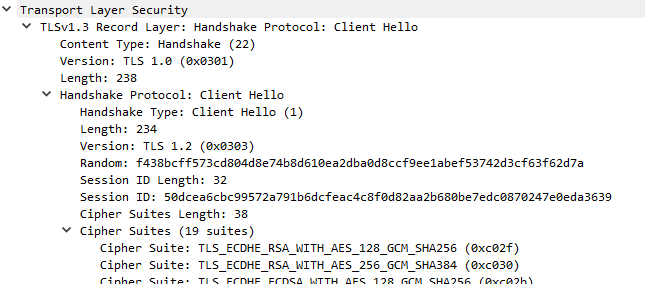
\includegraphics[width=\linewidth]{assets/oXq8RQt.png}
    \end{center}

    På bildet ser vi at klienten sender tjeneren en liste med 19 kryptografisuiter som 
    den kan velge mellom. Klienten sier også at den bruker TLS 1.2. Vi kan også se Random, som 
    er den genererte bytestringen.

    Tjeneren svarer så klienten med en Server Hello-pakke, som sier hvilken kryptografisuite 
    og TLS-versjon den har valgt, og som de begge kommer til å bruke fremover. Server Hello-pakken 
    sender \verb|server.crt| sertifikatet som vi genererte, og enda en tilfeldig generert bytestring 
    "Server Random".

    \begin{center}
        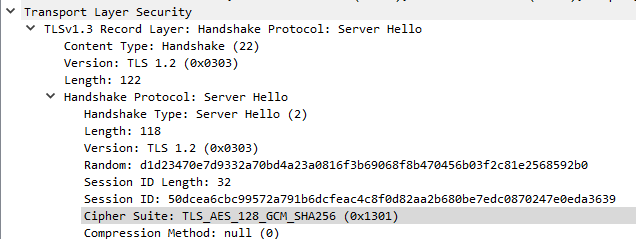
\includegraphics[width=\linewidth]{assets/6GQP3U2.png}
    \end{center}

    På bildet over ser vi Server Hello-pakken fra tjeneren til klienten.
    Vi kan se at den har valgt en kryptografisuite - \verb|TLS_AES_128_GCM_SHA256|,
    og at den har blitt enig med klienten om å bruke TLS 1.2. Vi ser også at den sender med
    en Random, som er den genererte bytestringen.

    Klienten genererer så enda en tilfeldig bytestring, som kalles en "premaster secret". Denne 
    blir kryptert ved bruk av den offentlige nøkkelen til tjeneren, som klienten får tak i via 
    sertifikatet som tjeneren sender. Klienten sender "premaster secret" til tjeneren, som kan 
    dekryptere den via den private nøkkelen, som tjeneren har. Tjeneren får så den krypterte 
    "premaster secret", og dekrypterer den. Etter dette så vil både klienten og tjeneren ha 
    en Client Random, Server Random og en Premaster Secret. Både klienten og tjeneren setter så 
    sammen disse tre tilfeldige bytestringene til en sesjonsnøkkel. Ettersom begge parter skal 
    ha alle de samme bytestringene, vil de ende opp med en lik sesjonsnøkkel.

    Klienten sender så en melding til tjeneren som sier at den har gjennomført det den 
    trenger for å begynne å overføre kryptert data, og tjeneren svarer med en melding som 
    sier det samme. Dette er en RSA-basert key-exchange.

    Når dette er gjort, er TLS-handshake gjennomført, og all data som blir sendt 
    vil nå være kryptert ved bruk av sesjonsnøkkelen og kryptografisuiten.
    Dersom vi ser på en tilfeldig valgt pakke med applikasjonsdata, ser vi 
    at det som blir overført ikke står i klartekst, men er kryptert. 

    \begin{center}
        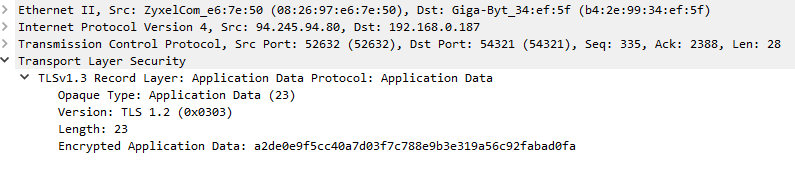
\includegraphics[width=\linewidth]{assets/81GWoEt.png}
    \end{center}

    Når det kommer til nedkobling, skjer akkurat det samme som skjer i 
    P3. Klienten kan skrive inn "exit" for å avslutte tilkoblingen. 
    Så gjennomgår klienten og tjeneren et nedkoblings-handshake, som 
    består av FIN og ACK-pakker. Grunnlaget for at vi ikke går dypt inn 
    i det i dette tilfellet er fordi, som sagt, det er nøyaktig det samme 
    som tjener-klient-programmet i P3.
\end{document}